\documentclass{article}%
\usepackage[T1]{fontenc}%
\usepackage[utf8]{inputenc}%
\usepackage{lmodern}%
\usepackage{textcomp}%
\usepackage{lastpage}%
\usepackage[head=40pt,margin=0.5in,bottom=0.6in]{geometry}%
\usepackage{graphicx}%
%
\title{\textbf{Malu Valeiro ejemplifica la sororidad con su obra}}%
\author{CAROLYN MANRIQUE}%
\date{04/03/2019}%
%
\begin{document}%
\normalsize%
\maketitle%
\textbf{URL: }%
http://www.eluniversal.com/entretenimiento/34355/malu{-}valeiro{-}ejemplifica{-}la{-}sororidad{-}con{-}su{-}obra\newline%
%
\textbf{Periodico: }%
EU, %
ID: %
34355, %
Seccion: %
entretenimiento\newline%
%
\textbf{Palabras Claves: }%
NO\_TIENE\newline%
%
\textbf{Derecho: }%
2.1%
, Otros Derechos: %
\newline%
%
\textbf{\textit{La artista textil fue ganadora del primer lugar del Premio Eugenio Mendoza, con la obra "La Regla de la Segunda Orden"}}%
\newline%
\newline%
%
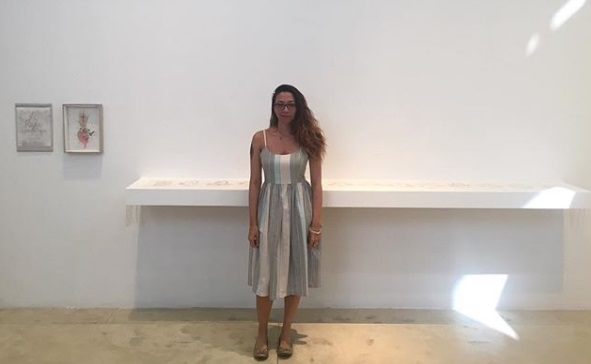
\includegraphics[width=300px]{EU_34355.jpg}%
\newline%
%
Basándose en la Segunda Orden franciscana, los artistas de origen, Malu Valeiro, presentó la obra La Regla de la Segunda Orden en la que hace un homenaje a 12 mujeres venezolanas que han sido víctimas de la violencia del género fuera del país. Esta fue la ganadora del primer lugar del Premio Eugenio Mendoza 2019, obteniendo una exposición individual en la Sala Mendoza para 2020 y una residencia artística en Cali, Colombia.~La artista comenzó en 2018 a estudiar la Segunda Orden escrita por Santa Clara, la primera obra basada en la orden creada "Por mujeres para mujeres", se basó en casos de femicidio íntimo en Venezuela. Usando la figura de las mártires en cada una de las víctimas. Esta pieza fue expuesta en el Centro Cultural BOD como parte del proyecto Arte y sociedad: jóvenes creadores venezolanos, creado por el Instituto Goethe.Para participar en el Salón Mendoza, Valeiro trabajó con 12 casos de mujeres venezolanas asesinadas fuera del país, la investigación fue realizada en mes y medio, la crisis migratoria ha causado que estos actos sean más frecuentes.~ ~La Regla de la Segunda Orden  ~es un libro textil, que muestra los 12 casos haciendo referencia a los 12 capítulos que conforman la Regla realizada por Santa Clara, además de lugar y fecha de nacimiento, muerte, nombre completo, foto y extractos de Las declaraciones de familiares y amigos que narran lo sucedido.~Según la Organización de las Naciones Unidas,~  137 mujeres alrededor del mundo mueren a manos de su pareja o de un miembro de su familiaVeleiro se ha encontrado con muchos casos, sin embargo, ha seleccionado más información, sobre el asesinato, su rostro y otros datos personales. Comenta que estos casos suelen quedar en el anonimato.~"Este es un ejercicio de afirmación, no puedo trabajar desde el anonimato, hay que darle un poco de dignidad", dice la artista.~{-}¿Considera su obra feminista?~{-}Para mi tema el feminismo es muy difícil, porque yo estoy como en el medio. Mis amigas feministas se sienten muy identificadas con mi trabajo; Sin embargo, yo no he asumido un artista feminista porque también tengo la convicción de que nuestro ejercicio como creadores es un ejercicio de interpelación. En esta obra hay unos elementos que también abordan el fenómeno actual de Venezuela, el tema de la diáspora y la estructura religiosa y católica. Personalmente me podría considerar postfeminista, una corriente que también cuestiona las propias bases del feminismo como movimiento político. Me siento más vinculado con la sororidad.En 2017 fueron asesinadas 87.000 mujeres en el planeta y más de la mitad fueron víctimas de personas cercanas. 30.000 fueron asesinados por su pareja, y otras 20.000 fueron asesinados por una familia.~La Regla de la Segunda Orden se encuentra exhibida en la Sala Mendoza, ubicada en la Universidad Metropolitana, al igual que el trabajo del resto de los participantes del premios y los ganadores de las menciones especiales.~"Es muy gratificante haber ganado un premio como este. Cada vez los artistas la tienen más difícil porque hay menos espacios", comenta Valeiro.~@carolynmanrique%
\newline%
%
\end{document}